%!TEX TS-program = xelatex
%\documentclass[]{resume}
\documentclass[]{resume}
\usepackage{graphicx}

\begin{document}

\graphicspath{ {images/} }

% --- Header --- %
\header{Michael\_}{Pobega}
       {Linux Systems Engineer}

% --- Footer --- %
\footer{References and Capstone documentation available upon request}

% --- Left Column --- %
\begin{aside}
  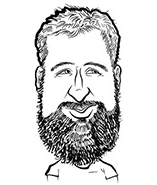
\includegraphics{caricaturesmall}
  \section{Contact}
    34 Ludlow St, Apt 20
    New York, NY 10002
    pobega@gmail.com
    (917) 436 - 0950
  \section{Skills}
    Linux system admin, 
    Kernel debugging,
    Shell scripting, Automation, Programming
  \section{Languages}
    Python, Perl, Bash,
    C/C++
  \section{Systems}
    Debian, Ubuntu, Gentoo,
    Arch, ChromiumOS
  \section{Tools}
	Ansible, Nagios, nmap, Git, nginx, Apache2, gdb, pdb, MySQL, MongoDB, Virsh, Qemu (KVM), Jenkins
  \section{Online}
    github.com/{\bodyfontbold pobega}
    linkedin.com/in/{\bodyfontbold pobega}
    serverfault.com/{\bodyfontbold pobega}
\end{aside}

% --- Right Column --- %
\begin{main}
  \section{Work Experience}
    \experience{Neverware}{New York, NY}{Software Developer}{September 2016 - Present}
      \point {Developer for Neverware's fork of ChromiumOS,  CloudReady}
      \point {Debugs and resolves hardware compatibility issues in CloudReady}
        \subpoint {Manages driver compatibility and patches hardware quirks in Linux kernel }
        \subpoint {Cherry-picks upstream changes into Longterm release kernels}
        \subpoint {Resolves hardware compatibility issues with CRAS ({\bodyfontitalics C}h{\bodyfontitalics R}omiumOS {\bodyfontitalics A}udio {\bodyfontitalics S}erver)}
      \point {Developed a tool to automate the creation of deployable CloudReady installer images}
        \subpoint {Uses Qemu and modifications to install scripts to automate a real install}
        \subpoint {Saves Neverware's support team 2 hours per customer request}
    \experience{Neverware}{New York, NY}{Site Reliability Engineer}{September 2014 - September 2016}
      \point {Administrator for Neverware's local Windows 7 Hypervisor solution, PCReady}
      \point {Administered roughly 300 PCReady servers across 120 schools}
        \subpoint {Troubleshot issues and worked with the dev team to identify root causes}
      \point {Engineered software for the monitoring and automation of PCReady tasks}
      \point {Solely managed customer support interactions for PCReady}
    \experience{SUNYIT ITS Department}{Utica, NY}{Linux System Administrator}{September 2013 - May 2014}
      \point {Worked with the Administration team to deploy and administer Linux servers}
      \point {Migrated services running on legacy Unix software/hardware to a virtualized environment}
        \subpoint {Migrated primarily from ancient Sun Solaris server}
      \point {Reimplemented logic of expensive mailing list software in Perl}
        \subpoint {Solution integrated with their existing LDAP (authentication) setup}
      \point {Introduced configuration management through Ansible as a tool for rapid redeployment}
        \subpoint {Implemented a majority of existing server configurations in Ansible Playbooks}
    \experience{SUNYIT CS Department}{Utica, NY}{Junior System Administrator}{January 2010 - January 2012}
      \point {Responsible for the Gentoo Linux lab, as well as other misc. Linux labs on campus}
      \point {Maintained \& updated Gentoo master image}
        \subpoint {Image was deployed to labs via PXE boot multicast imaging process.}
      \point {Implemented multicast ISO burning solution in Bash (\textit{wodimcast})}
  \hrulefill
  \section{Education}
    \experience{SUNY Institute of Technology}{Utica, NY}{BSc Computer Science}{Class of May 2014}
      \point {Deployed and configured Nagios to monitor pre-existing SUNYIT production services}
      \point {Set up Ansible configuration management on production network}
        \subpoint {Used to deploy 'Nagios Remote Plugin Executor'}
        \subpoint {Automated Nagios related tasks, simplifying administration}
\end{main}

\end{document}
